\documentclass[17pt]{beamer}
%\documentclass[handout]{beamer} %Makes Handouts
\usetheme{Singapore} %Gray with fade at top
\useoutertheme[subsection=false]{miniframes} %Supppress subsection in header
\useinnertheme{rectangles} %Itemize/Enumerate boxes
\usecolortheme{seagull} %Color theme
\usecolortheme{rose} %Inner color theme

\definecolor{light-gray}{gray}{0.75}
\definecolor{dark-gray}{gray}{0.55}
\setbeamercolor{item}{fg=light-gray}
\setbeamercolor{enumerate item}{fg=dark-gray}

\setbeamertemplate{navigation symbols}{}
\setbeamertemplate{mini frames}{}
%\setbeamercovered{dynamics}
\setbeamerfont*{title}{size=\Large,series=\bfseries}
\setbeamerfont{footnote}{size=\tiny}

%\setbeameroption{notes on second screen} %Dual-Screen Notes
%\setbeameroption{show only notes} %Notes Output

\setbeamertemplate{frametitle}{\vspace{.5em}\bfseries\insertframetitle}
\newcommand{\heading}[1]{\noindent \textbf{#1}\\ \vspace{1em}}
\newcommand{\questions}{\frame{{\large Questions?}}}

\usepackage{bbding,color,multirow,times,ccaption,tabularx,graphicx,verbatim,booktabs}
\usepackage{colortbl} %Table overlays
\usepackage[english]{babel}
\usepackage[latin1]{inputenc}
\usepackage[T1]{fontenc}
\usepackage{lmodern}
\usepackage{alltt}

\usepackage{tikz}
\usetikzlibrary{shapes,arrows,decorations.pathreplacing,calc}


\author[]{Thomas J. Leeper}
\institute{
  Government Department\\London School of Economics and Political Science
}


\title{Survey Experiments in Context}

\date[]{}

\begin{document}

\frame{\titlepage}


\section{Introductions}
\frame{\tableofcontents[currentsection]}

\frame{
\frametitle{Who am I?}

\small

\begin{itemize}\itemsep0.5em

\item Thomas Leeper

\item Assistant Professor in Political Behaviour at London School of Economics

\begin{itemize}
\item Originally from Minnesota, USA
\item PhD from Northwestern University (Chicago, USA)
\item Worked At Aarhus University (Denmark) for 2.5 years
\end{itemize}

\item Interested in public opinion and political psychology

\item Email: \href{mailto:t.leeper@lse.ac.uk}{t.leeper@lse.ac.uk}

\end{itemize}

}


\frame{

\frametitle{Activity!}

\only<2-4,6>{
\begin{enumerate}
\item<2-4,6> Ask you to guess a number
\item<3-4,6> Number off 1 and 2 across the room
\item<4,6> Group 2, close your eyes
\item<6> Group 1, close your eyes
\end{enumerate}
}

\Large
\only<5>{\textit{Group 1}\\ Think about whether the population of Chicago is more or less than 500,000 people. What do you think the population of Chicago is?}
\only<7>{\textit{Group 2}\\ Think about whether the population of Chicago is more or less than 10,000,000 people. What do you think the population of Chicago is?}

}

\frame{}

\frame{

\frametitle{Enter your data}

\begin{itemize}\itemsep1em
\item Go here: \url{http://bit.ly/297vEdd}
\item Enter your guess and your group number
\end{itemize}


%\url{http://goo.gl/forms/xDW4FLm9pau0O8zz2}

}


\frame{

\frametitle{Results}

\begin{itemize}\itemsep1em
\item True population: 2.79 million
\item<2-> What did you guess? \href{https://docs.google.com/spreadsheets/d/1SKWljS1EeNkAV5V0NZUwrKOu3LQFILVMB37xfTxyrPM/edit?usp=sharing}{(See Responses)}
\item<3-> What's going on here?
	\begin{itemize}
	\item An experiment!
	\item Demonstrates ``anchoring'' heuristic
	\end{itemize}
\item<4-> Experiments are easy to analyze, but difficult to design
\end{itemize}

}



\frame{

\frametitle{Who are you?}

\begin{itemize}\itemsep1em

\item Introduce yourself to a neighbour

\item Where are you from?

\item What do you hope to learn from the course?

\end{itemize}

}



\frame{

\frametitle{Quick Survey}

\begin{enumerate}\itemsep0.5em
\item<2-> How many of you have worked with survey data before?
\item<3-> Of those, how many of you have \textit{performed} a survey before?
\item<4-> How many of you have worked with experimental data before?
\item<5-> Of those, how many of you have \textit{performed} an experiment before?
\end{enumerate}

}



\section{Course Outline}
\frame{\tableofcontents[currentsection]}


\frame{

\frametitle{Course Materials}

\begin{center}
All material for the course is available at:\\

\url{http://www.thomasleeper.com/surveyexpcourse}
\end{center}

}

\frame{

\frametitle{Learning Outcomes}

\small

By the end of the week, you should be able to\dots

\begin{enumerate}
\item<2-> Explain how to analyze experiments quantitatively.
\item<3-> Explain how to design experiments that speak to relevant research questions and theories.
\item<4-> Evaluate the uses and limitations of several common survey experimental paradigms.
\item<5-> Identify practical issues that arise in the implementation of experiments and evaluate how to anticipate and respond to them.
\end{enumerate}

}


\frame{

\frametitle{Schedule of Five Sessions}

\begin{enumerate}\itemsep0.5em
\item Survey Experiments in Context
\item Examples and Paradigms
\item External Validity
\item Sources of Heterogeneity
\item Lingering Issues
\end{enumerate}

}


\questions



\section[History]{History of Experiments}
\frame{\tableofcontents[currentsection]}

\frame{

\frametitle{Experiments}

\begin{itemize}
\item Oxford English Dictionary defines ``experiment'' as:

\begin{enumerate}
\item A scientific procedure undertaken to make a discovery, test a hypothesis, or demonstrate a known fact
\item A course of action tentatively adopted without being sure of the outcome
\end{enumerate}

\item Thus, ``experiments'' have a very long history

\item Major advances in design and analysis of experiments based on agricultural and later biostatistical research in the 19th century
	\begin{itemize}
	\item R.A. Fisher
	\item Jerzy Neyman
	\item Karl Pearson
	\item Oscar Kempthorne
	\end{itemize}

\end{itemize}

}

\frame{

\frametitle{In Social Sciences}

\begin{itemize}
\item ``Experiments'' emerged in psychology 19th century
	\begin{itemize}
	\item Not randomized -- more like ``What if?'' studies
	\item Heavily laboratory-based or clinical
	\end{itemize}
\item First randomized, controlled trial (RCT) by Peirce and Jastrow in 1884
\item RCTs actually came much later to medicine (mid-20th century)
\item And have been a major part of the ``credibility revolution'' in economics
	\begin{itemize}
	\item See, especially, LaLonde (1986)
	\end{itemize}
\end{itemize}

}


\frame{

\frametitle{In Political Science I}

\begin{itemize}
\item American Political Science Association president A. Lawrence Lowell (1922): 
\begin{quote}
We are limited by the impossibility of experiment. Politics is an observational, not an experimental science\dots
\end{quote}
\item First ``experiment'' by Harold Gosnell (1924)
\item King, Keohane, and Verba (1994) only mentions experiments once
\item Gerber and Green (2000) first major \textit{field} experiment
\end{itemize}

}

\frame{

\frametitle{In Political Science II}

\begin{itemize}
\item Behavioral revolution of 1940s/1950s brought survey research to prominence
\item Experiments were being performed in laboratories but not elsewhere
\item Survey research was not experimental because interviewing was still mostly paper-based
\item 1983: Merrill Shanks and the Berkeley Survey Research Center develop CATI
\item Paul Sniderman and Tom Piazza performed the first, simple survey experiment\footnote{Sniderman, Paul M., and Thomas Piazza. 1993. The Scar of Race. Cambridge, MA: Harvard University Press.}
\item They then created the ``first multi-investigator''
\item Skip Lupia and Diana Mutz used that model to create TESS
\end{itemize}

}


\questions



\section[Logic]{Logic of Experiments}
\frame{\tableofcontents[currentsection]}


\frame{
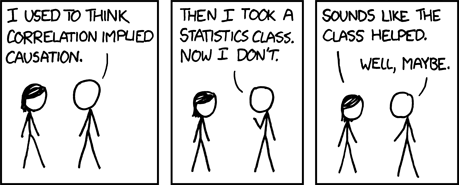
\includegraphics[width=\textwidth]{images/correlation.png}
}


\frame{

\frametitle{Addressing Confounding}

In observational research\dots

\begin{enumerate}\itemsep0.5em
\item<2-> Correlate a ``putative'' cause ($X$) and an outcome ($Y$)
\item<3-> Identify all possible confounds (\textbf{Z})
\item<4-> ``Condition'' on all confounds
	\begin{itemize}
	\item Calculate correlation between $X$ and $Y$ at each combination of levels of \textbf{Z}
	\end{itemize}
\item<5-> Basically:\\
$Y = \beta_0 + \beta_1 X + \beta Z + \epsilon $
\end{enumerate}

}

\frame{

\frametitle{Experiments are different}

\begin{enumerate}
\item<2-> They require us to think carefully about causality
\item<3-> Draw causal inferences through \textit{design} not \textit{analysis}
\item<4-> Experiments reveal ``counterfactuals'' or ``potential outcomes''
\item<5-> We define a ``causal effect'' as the difference between two potential outcomes
\end{enumerate}

}


% Mill's method of difference
\frame{
\frametitle{{\normalsize Mill's Method of Difference}}

\small

If an instance in which the phenomenon under investigation occurs, and an instance in which it does not occur, have every circumstance save one in common, that one occurring only in the former; the circumstance in which alone the two instances differ, is the effect, or cause, or an necessary part of the cause, of the phenomenon.
}



\frame{

\frametitle{Definitions}

\begin{itemize}
\item<2-> Unit: A physical object at a particular point in time

\item<3-> Treatment: An intervention, whose effects we wish to assess relative to some other (non-)intervention

\item<4-> Potential outcomes: The outcome for each unit that we would observe if that unit received each treatment

	\begin{itemize}
	\item Multiple potential outcomes for each unit, but we only observe one of them
	\end{itemize}

\item<5-> Causal effect: The comparisons between the unit-level potential outcomes under each intervention
\end{itemize}
}





% Causal graphs

\begin{frame}
\begin{center}
\begin{tikzpicture}[>=latex',circ/.style={draw, shape=circle, node distance=5cm, line width=1.5pt}]
    \draw (0,0) node[left] (X) {\textcolor<2->{red}{Smoking}};
    \draw[->] (X) -- (5,0) node[right] (Y) {Cancer};
    \draw[->] (-3,3) node[above] (Z) {Sex} -- (X);
    \draw[->] (Z) -- (Y);
    \draw[->] (5,2) node[above] (A) {Environment} -- (Y);
    \draw[->] (4,-3) node[below, text width=3cm, align=center] (E) {Genetic\\Predisposition} -- (Y);
    \draw[->] (-2, -2) node[below, text width=2.5cm, align=center] (W) {Parental\\Smoking} -- (X);
    \draw[->] (W) -- (Y);
    \draw<2->[->, dashed, very thick] (E) -- (X);
\end{tikzpicture}
\end{center}
\end{frame}




% Individual-level effects versus ATEs


\frame{
	\frametitle{The Experimental Ideal}
	\small
	A randomized experiment, or randomized control trial is:
 		\begin{quote}\small
 			The observation of units after, and possibly before, a randomly assigned intervention in a controlled setting, which tests one or more precise causal expectations
 		\end{quote}
 	This is Holland's ``statistical solution'' to the fundamental problem of causal inference
}

\frame{
\frametitle{The Experimental Ideal}
\begin{itemize}\itemsep0.5em
\item It solves both the temporal ordering and confounding problems
	\begin{itemize}
   		\item Treatment ($X$) is applied by the researcher before outcome ($Y$)
   		\item Randomization means there are no confounding ($Z$) variables
	\end{itemize}
\item Thus experiments are a ``gold standard'' that always provides causal inference
\item<5-> Basically:\\
$Y = \beta_0 + \beta_1 X + \epsilon $
\end{itemize}
}


\frame{

\frametitle{Neyman-Rubin Potential Outcomes Framework}

If we are interested in some outcome $Y$, then for every unit $i$, there are numerous ``potential outcomes'' $Y*$ only one of which is visible in a given reality

Concisely, we typically discuss two potential outcomes:

\begin{itemize}
\item $Y_{0i}$, the \textit{potential} outcome that would be \textit{realized} if $X_i = 0$ (assigned to control)
\item $Y_{1i}$, the \textit{potential} outcome that would be \textit{realized} if $X_i = 1$ (assigned to treatment)
\end{itemize}

We are only able to see one of these potential outcomes for each unit.

}


\frame{

\frametitle{Aside}

\begin{itemize}
\item The history of the potential outcomes framework is contested
\item Most people attribute it to Donald Rubin
\item Paul Holland was the first to link to the philosophical discussions of causality
\item Donald Rubin attributes this to Jerzy Neyman (1923)
\item James Heckman denies all of this and attributes it Andrew Roy (1951)
\end{itemize}
}




\frame{
	\frametitle{Random Assignment}

\small
\begin{itemize}\itemsep0.5em
\item A physical process of randomization
\item Breaks the ``selection process''
	\begin{itemize}\small
	\item Units only take value of $X$ because of assignment
	\end{itemize}
\item This means:
	\begin{itemize}\small
	\item All covariates are balanced between groups
	\item Potential outcomes are balanced between groups
	\item In sum: No confounding
	\end{itemize}
\end{itemize}

}

\begin{frame}
\small 
\begin{center}
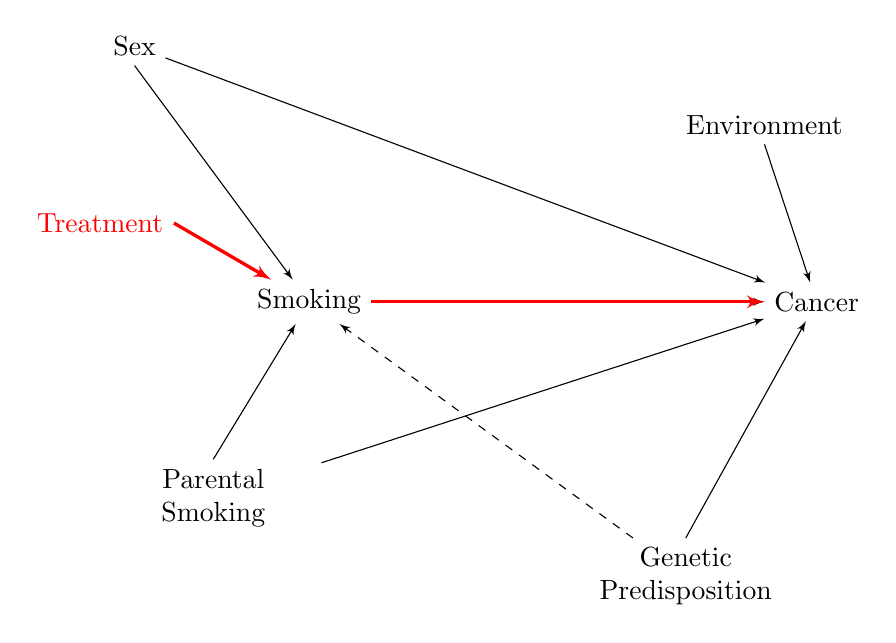
\begin{tikzpicture}[>=latex',circ/.style={draw, shape=circle, node distance=5cm, line width=1.5pt}]
    \draw[->] (0,0) node[left] (X) {Smoking} -- (5,0) node[right] (Y) {Cancer};
    \draw[->] (-3,3) node[above] (Z) {Sex} -- (X);
    \draw[->] (Z) -- (Y);
    \draw[->] (5,2) node[above] (A) {Environment} -- (Y);
    \draw[->] (4,-3) node[below, text width=3cm, align=center] (E) {Genetic\\Predisposition} -- (Y);
    \draw[->] (-2, -2) node[below, text width=2.5cm, align=center] (W) {Parental\\Smoking} -- (X);
    \draw[->] (W) -- (Y);
    \draw[->, dashed] (E) -- (X);
    
    \draw<2->[->, very thick, color=red] (-2.5,1) node[left, color=red] (Tr) {Treatment} -- (X);
    \draw<2->[->, very thick, color=red] (X) -- (Y);
\end{tikzpicture}
\end{center}
\end{frame}



% design-based experimental inference
\frame{
	\frametitle{Experimental Inference I}
	\small
	\begin{itemize}\itemsep0.5em
    	\item<1-> Causal inference is a comparison of two \textit{potential outcomes}
    	\item<2-> A potential outcome is the value of the outcome (Y) for a given unit (i) after receiving a particular version of the treatment (X)
    	\item<3-> Each unit has multiple \textit{potential} outcomes, but we only observe one of them
    	\item<4-> A \textit{causal effect} is the difference between these (e.g., $Y_{X=1} - Y_{X=0}$), all else constant
	\end{itemize}
}

\frame{
	\frametitle{Experimental Inference II}
	\small
	\begin{itemize}\itemsep0.5em
    	\item<1-> We cannot see individual-level causal effects
    	\item<2-> We can see \textit{average causal effects}
    		\begin{itemize}
        		\item<2-> Ex.: Average difference in cancer between those who do and do not smoke
    		\end{itemize}
    	\item<3-> We want to know: $TE_i = Y_{1i} - Y_{0i}$
	\end{itemize}
}

\frame{
	\frametitle{Experimental Inference III}
	\small
	\begin{itemize}\itemsep0.5em
		\item<1-> We want to know: $TE_i = Y_{1i} - Y_{0i}$ for every $i$ in the population
		\item<2-> We can average: $ATE = E[Y_{1i} - Y_{0i}] = E[Y_{1i}] - E[Y_{0i}]$
		\item<3-> But we still only see one potential outcome for each unit:\\ \vspace{1em}
    		$ATE_{naive} = E[Y_{1i} | X = 1] - E[Y_{0i} | X = 0]$
    	\item<4-> Is this what we want to know?
	\end{itemize}
}


\frame{
	\frametitle{Experimental Inference IV}
	\small
	\begin{itemize}\itemsep0.5em
	\item What we want and what we have:
		\begin{align}
		ATE & = E[Y_{1i}] - E[Y_{0i}] \\[1em]
		ATE_{naive} & = E[Y_{1i} | X = 1] - E[Y_{0i} | X = 0]
		\end{align}		
	\item<2-> Are the following statements true?\\
  		\begin{itemize}\itemsep0.5em
      		\item<2-> $E[Y_{1i}] = E[Y_{1i} | X = 1]$
      		\item<2-> $E[Y_{0i}] = E[Y_{0i} | X = 0]$
  		\end{itemize}
  	\item<3-> Not in general!
  	\end{itemize}
}

\frame{
	\frametitle{Experimental Inference V}
	\small
	\begin{itemize}\itemsep0.5em
    	\item Only true when both of the following hold:
    	\begin{align}
    	E[Y_{1i}] = E[Y_{1i} | X = 1] = E[Y_{1i} | X = 0]\\
    	E[Y_{0i}] = E[Y_{0i} | X = 1] = E[Y_{0i} | X = 0]
    	\end{align}
    	\item In that case, potential outcomes are \textit{independent} of treatment assignment
		\item If true, then:
    	\begin{align*}
    	ATE_{naive} & = E[Y_{1i} | X = 1] - E[Y_{0i} | X = 0] \tag{5}\\
    	& = E[Y_{1i}] - E[Y_{0i}]\\
    	& = ATE
    	\end{align*}
	\end{itemize}
}

\frame{
	\frametitle{Experimental Inference VI}
	\small
	\begin{itemize}\itemsep0.5em
    	\item This holds in experiments because of randomization
   		\item Units differ only in what side of coin was up
  		\item Experiments randomly reveal potential outcomes
  		\item This means there is no confounding (selection bias)
	\end{itemize}
}


\frame{
	\frametitle{``The Perfect Doctor''}

\small
\begin{center}
\begin{tabular}{ccc}
Unit & $Y_0$ & $Y_1$ \\ \hline 
1 & ? & ? \\
2 & ? & ? \\
3 & ? & ? \\
4 & ? & ? \\
5 & ? & ? \\
6 & ? & ? \\
7 & ? & ? \\
8 & ? & ? \\ \hline
\textbf{Mean} & \textbf{?} & \textbf{?} \\
\end{tabular}
\end{center}
}

\frame{
	\frametitle{``The Perfect Doctor''}

\small
\begin{center}
\begin{tabular}{ccc}
Unit & $Y_0$ & $Y_1$ \\ \hline 
1 & ? & 14 \\
2 & 6 & ? \\
3 & 4 & ? \\
4 & 5 & ? \\
5 & 6 & ? \\
6 & 6 & ? \\
7 & ? & 10 \\
8 & ? & 9 \\ \hline
\textbf{Mean} & \textbf{5.4} & \textbf{11} \\
\end{tabular}
\end{center}
}

\frame{
	\frametitle{``The Perfect Doctor''}

\small
\begin{center}
\begin{tabular}{ccc}
Unit & $Y_0$ & $Y_1$ \\ \hline 
1 & 13 & 14 \\
2 & 6 & 0 \\
3 & 4 & 1 \\
4 & 5 & 2 \\
5 & 6 & 3 \\
6 & 6 & 1 \\
7 & 8 & 10 \\
8 & 8 & 9 \\ \hline
\textbf{Mean} & \textbf{7} & \textbf{5} \\
\end{tabular}
\end{center}
}



\frame{
\frametitle{Experimental Analysis I}
\small
\begin{itemize}
\item The statistic of interest in an experiment is the \textit{sample average treatment effect} (SATE)
\item If our sample is \textit{representative}, then this provides an estimate of the population average treatment (PATE)
\item This boils down to being a mean-difference between two groups:
	\begin{equation}
	SATE = \frac{1}{n_1}\sum Y_{1i} - \frac{1}{n_0}\sum Y_{0i}
	\end{equation}
\item In practice we often estimate this using t-tests, ANOVA, or OLS regression
\end{itemize}
}





\frame{
\frametitle{Experimental Analysis II}
	\small
\begin{itemize}\itemsep0.5em
\item We don't just care about the size of the SATE. We also want to know whether it is significantly different from zero (i.e., different from no effect/difference)
\item To know that, we need to estimate the \textit{variance} of the SATE
\item The variance is influenced by:
	\begin{itemize}
	\item Total sample size
	\item Variance of the outcome, $Y$
	\item Relative size of each treatment group
	\end{itemize}
\end{itemize}
}

\frame{
\frametitle{Experimental Analysis III}
	\small
\begin{itemize}\itemsep0.5em
\item Formula for the variance of the SATE is:\\
$\widehat{Var}(SATE) = \dfrac{\widehat{Var}(Y_0)}{N_0} + \dfrac{\widehat{Var}(Y_1)}{N_1}$

	\begin{itemize}
	\item $\widehat{Var}(Y_0)$ is control group variance
	\item $\widehat{Var}(Y_1)$ is treatment group variance
	\end{itemize}

\item We often express this as the \textit{standard error} of the estimate:\\
$\widehat{SE}_{SATE} = \sqrt{\frac{\widehat{Var}(Y_0)}{N_0} + \frac{\widehat{Var}(Y_1)}{N_1}}$
\end{itemize}
}


\frame{

\frametitle{Intuition about Variance}

\begin{itemize}
\item Bigger sample -\textgreater{} smaller SEs
\item Smaller variance -\textgreater{} smaller SEs
\item Efficient use of sample size:
	\begin{itemize}
	\item When treatment group variances equal, equal sample sizes are most efficient
	\item When variances differ, sample units are better allocated to the group with higher variance in \emph{Y}
	\end{itemize}
\end{itemize}


}


\frame[fragile]{

\begin{verbatim}
# theoretical randomizations
d <- data.frame(y1 = c(14,0,1,2,3,1,10,9), 
                y0 = c(13,6,4,5,6,6,8,8) )

onedraw <- function(eff=FALSE, dat = d){
  r <- replicate(nrow(dat), sample(1:2,1))
  dat[cbind(1:nrow(dat),r)] <- NA
  if (eff) {
    return(mean(dat[,'y1'], na.rm=TRUE) -
           mean(dat[,'y0'], na.rm=TRUE) )
  } else {
    return(dat)
  }

onedraw() # one randomization
onedraw(TRUE) # one effect estimate

# simulate 2000 experiments from these data
x1 <- replicate(2000, onedraw(TRUE))
hist(x1, col=rgb(1,0,0,.5), border='white')
abline(v=-2, lwd=3, col='red') # true effect
\end{verbatim}

}



\frame{

\frametitle{Statistical Power}

\begin{itemize}
\item Power analysis to determine sample size
\item Type I and Type II Errors
	\begin{itemize}
	\item True positive rate is power
	\item False negative rate is the significance threshold ($\alpha$)
	\end{itemize}
\end{itemize}

\begin{tabular}{lrr}
\toprule
& \textbackslash{}(\ H\_0\ \textbackslash{}) True & \textbackslash{}(\ H\_0\ \textbackslash{}) False \\ \midrule
Reject \textbackslash{}(\ H\_0\ \textbackslash{}) & Type 1 Error & \textbf{True positive} \\
Accept \textbackslash{}(\ H\_0\ \textbackslash{}) & False negative & Type II error \\ \bottomrule
\end{tabular}

}

\frame{

\frametitle{Doing a Power Analysis}

\begin{itemize}
\item $\mu$, Treatment group mean outcomes
\item $N$, Sample size
\item $\sigma$, Outcome variance
\item $\alpha$ Statistical significance threshold
\item $\phi$, a sampling distribution
\end{itemize}

$Power = \phi\left( \frac{|\mu_1 - \mu_0|\sqrt{N}}{2\sigma} - \phi^{-1}\left( 1 - \frac{\alpha}{2} \right) \right)$

}





\frame{
\frametitle{Intuition about Power}

Minimum detectable effect is the smallest effect we could detect given sample size, ``true'' effect size, variance of outcome, power, and $\alpha$

\begin{center}
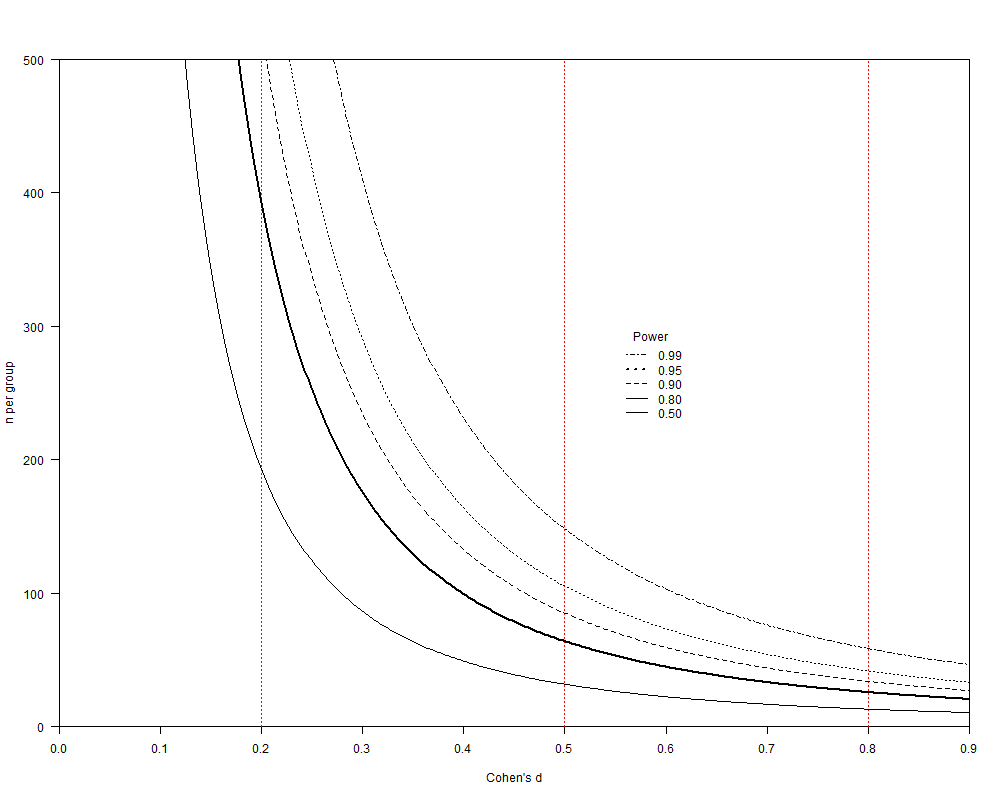
\includegraphics[height=0.85\textheight, trim = 0in 0in 0in 0.5in , clip]{images/power}
\end{center}

% Sometimes non-zero effects are not detectable
% Talk about Gelman and Stern

}


\frame{

\frametitle{Substantive effect sizes}

\begin{itemize}
\item We rarely care only about statistical significance
	\begin{itemize}
	\item Know if effects are large or small
	\item Compare effects across studies
	\end{itemize}
\item Cohen's $d$:\\ $d = \frac{\bar{x}_1 - \bar{x}_0}{s}$, where
$s = \sqrt{\frac{(n_1 - 1)s_1^2 + (n_0 - 1)s_0^2}{n_1 + n_0 - 2}}$
\item Small: 0.2; Medium: 0.5; Large: 0.8
\end{itemize}

}


\frame{

\frametitle{Aside: Complex Designs}

\begin{itemize}
\item An experiment can have any number of conditions
	\begin{itemize}
	\item Up to the limits of sample size
	\item More than 8--10 conditions is typically unwieldy
	\end{itemize}
\item Typically analyze complex designs using ANOVA or regression, but we are still ultimately interested in pairwise comparisons to estimates SATEs
	\begin{itemize}
	\item Treatment--treatment, or treatment-control
	\item Without control group, we don't know which treatment(s) affected the outcome
	\end{itemize}
\end{itemize}

}


\frame{}


\frame{
\frametitle{\textit{Survey}-experiments, specifically}

\begin{itemize}
\item Everything so far applies to any kind of experiment
\item<2-> A survey experiment is just an experiment that occurs in a survey context
	\begin{itemize}
	\item As opposed to in the field or in a laboratory
	\end{itemize}
\item<3-> Sometimes a distinction is made between survey and online experiments
\item<4-> Lots of common paradigms for survey experiments (tomorrow)
\end{itemize}
}


\frame{

\frametitle{Combining \textit{Survey Design} and\\ \textit{Experimental Design}}

\begin{itemize}\itemsep1em
\item Sample is representative of population in every respect (in expectation)
\item Sample Average Treatment Effect (SATE) is the average of the sample's individual-level treatment effects
	\begin{itemize}
	\item Unbiased estimate of PATE
	\end{itemize}
\item<2-> Says nothing about effect heterogeneity
	\begin{itemize}
	\item Design is optimized for estimating SATE
	\item Discuss this on Wednesday
	\end{itemize}
\end{itemize}
}


\questions


\frame{

\frametitle{Homework!}

\begin{itemize}
\item Get a sense of what can be studied experimentally
\item Visit Time-Sharing Experiments for the Social Sciences
	\begin{itemize}
	\item \url{http://tessexperiments.org}
	\end{itemize}
\item Pick two studies from TESS
\item We will share them in class tomorrow
\end{itemize}

}


\appendix
\frame{}

\end{document}
